% Visually separate introduction from other front matter items
% \addtocontents{toc}{\protect\bigskip}

\chapter{Introduction}
% \addcontentsline{toc}{chapter}{\textsc{Introduction}}
\label{chapter:introduction}

A compelling challenge for many scientific fields is finding ways to influence systems, so they exhibit a desired behavior. Biology is no exception. Finding a cure to a disease is essentially finding a way to control the system of the human body to get rid of the disease. Of course, today, we are not yet able to make a single complete model of the human body, but we still can make models of some of its parts, such as gene-protein interactions in a cell~\cite{Cardelli2005}. 

The available cell models are also very useful for curing diseases. For example, we can try to find a way to reprogram a cancer cell into a healthy one or to reprogram a stem cell into a phenotype (a specific cell type) that is needed for regenerative medicine. The problem of controlling a cell is called \emph{cell reprogramming}, and it is one of the most significant challenges of regenerative medicine~\cite{Cherry2012}. In practice, reprogramming strategies often rely on targeted perturbations of gene expression, including forced over-expression, or knockout, implemented through methods such as CRISPR-based technologies~\cite{Doudna2014} and RNA interference~\cite{Fire1998}.


% In biology, the state into which a system evolves is commonly referred to as \emph{phenotype}~\cite{Cheng2016}. It is a set of observable characteristics of an organism. Therefore, in biology, the goal of control is to drive a system into the desired phenotype. 

% Sys. biology modelling
% The focus of this work is on the control of biological systems. 
% Therefore, the problem falls into the scope of the \emph{systems biology} field where the aim is to apply formal methods developed by computer science to the biological models. The current focus of systems biology is on the cellular level as it is the basis of biological systems and even this basic level is still considered difficult to model as there might be hundreds of interactions in the play. The task of controlling cells is called \emph{cell reprogramming}, and it is one of the most significant challenges of regenerative medicine~\cite{Cherry2012}.

% BNs
To study and design such interventions, we rely on field of \emph{systems biology} that aims to apply formal methods developed by computer science to biological models. Systems biology uses a variety of models ranging from discrete (e.g. Boolean networks~\cite{Schwab2020}), through continuous (e.g. ODE~\cite{Gratie2013}), to hybrid models~\cite{Grossman1993}. A very efficient model to capture numerous interactions at the cellular level is \emph{Boolean network} (BN) because this model is both simple and expressive. Moreover, BNs have applications in many other areas, including circuit theory and behavioral science~\cite{Roli2015, Kochemazov2014}. 

BNs are composed of two parts: a finite set of Boolean \emph{variables} representing genes or other biochemical substances and \emph{update functions} which specify the way variables dynamically change their value based on influences from other variables. BNs generate a finite discrete state-space which makes them convenient for computational analyses. When starting from any initial state, the BN eventually establishes in some single state or a set of states. These components of BN state space are called \emph{attractors}. They can be viewed as an abstraction for phenotypes of the modeled biological systems~\cite{Cheng2016}.


% Control
A computational model is considered controllable if we can assure that from some initial state, it reaches a desired final state in a finite amount of steps. When controlling BNs, we are interested in BN reaching the desired attractor. This property is well-studied in the context of BNs without unknown parts~\cite{Zanudo2015, Mandon2019CMSB, Su2020BCB, Fontanals2020}. However, the problem has not received a lot of attention in the partially specified setting yet, that allows to capture the uncertainty in the model typical for biological systems~\cite{Zou2013, Benes2019}. 

The definition of control is rather broad and allows many variations of the problem for BNs. To change the normal behavior of BN, understandably, we need to interfere with the model in some way. We call these interventions \emph{perturbations}. However, we can consider many types of perturbations. They vary in three aspects. Firstly, we can either fix variable values to some fixed value or change the rules of their evolution. Secondly, we can apply the perturbation just as a single transition step (e.g. a brief exposure to a signalling molecule), or we can hold the perturbations for more transition steps (e.g. a prolonged drug treatment), but even permanent perturbations (e.g. a CRISPR-mediated gene knockout) are considered. Lastly, the perturbation can be applied only once, or we consider applying perturbations and releasing perturbations at any time.

Apart from the different kinds of perturbations, control problems also vary in terms of the objective. Four common control goals are: (i) driving the system from a specified source state to a specified target attractor (\emph{source-target control})~\cite{Su2019CMSB}, (ii) achieving a single desired target attractor irrespective of the current state (\emph{target control})~\cite{Kim2013}, (iii) achieving control between every pair of attractors (\emph{full control})~\cite{Fiedler2013}, and (iv) reaching the set of states satisfying given conditions (\emph{phenotype control})~\cite{Fontanals2020}. For instance, source-target control may consist in driving a proliferating cell to an apoptotic attractor; target control would require driving the system to the same apoptotic attractor from \emph{any} initial cellular state; full control may correspond to the ability to switch the system among all stable cell fates represented by attractors, such as proliferation, quiescence, and apoptosis; and phenotype control may correspond to steering the network to any state satisfying a prescribed pattern of marker activity, for example states in which stemness genes are inactive, and differentiation markers are active.

% ParBNs
In practice, the exact Boolean functions of the model may not be precisely known due to various uncertainties such as insufficient experimental knowledge~\cite{Grieco2013}, inconsistent observations~\cite{Geris2016}, genetic mutations~\cite{Martin2016}, or any other ambiguities. In contrast, there is typically good evidence of the fact that a variable regulates another one. This issue can be addressed by allowing BNs to contain function symbols. \emph{Partially specified Boolean networks} (\PBN{s})~\cite{Zou2013, Benes2019} allows to specify only regulators of a variable and thus capture multiple variants of the possible actual behavior of variables without conducting many more expensive experimental observations. Every interpretation of the unknown parts can be understood as an instance of a standard BN. The number of these instances can be doubly exponential in the worst case~\cite{Wang2012}. 

% PSBNs control challenges
The partially specified setting brings many new challenges to the control problem. First, the nature of BN state transition graph may change dramatically between the interpretations~\cite{Benes2019,aeon}. Even the original goal of the standard control -- to stabilize in a target attractor -- might not be feasible in some instances as the given attractor is not present in them. 
Secondly, the BN control problem is optimizing -- we are trying to minimize the number of perturbations done to a network, while we must guarantee that the target attractor is reached in all BN non-deterministic runs. It was shown that for many biological models, controlling values of only a few variables is sufficient to drive the network into any attractor of the BN~\cite{Zanudo2015}. On the contrary, this is usually not the case for the \PBN{s}. Due to the uncertainties, we would often need to fix the value of many variables to guarantee \PBN{} to reach the given attractor in all network instances. Such an approach is not applicable in practice as each perturbation can be very costly in the real environment. Therefore, the optimization criteria should be adjusted.


In our current research line, we decided to treat the interpretations solely as unknown knowledge and consider only the state perturbations that fix the value of variables. To cope with minimization criteria, the output of the control problem for \PBN{} is a complete \emph{mapping} from the domain of perturbations to the domain of relevant interpretations. This way, it is possible to manually explore the available perturbations and consider both the cost of perturbation and the \emph{robustness} of perturbation -- the proportion of interpretations for which the perturbation ensures \PBN{} stabilization in the given attractor with all considered interpretations.

\section{Contribution}

\begin{figure}[htbp!]
    \centering
    
    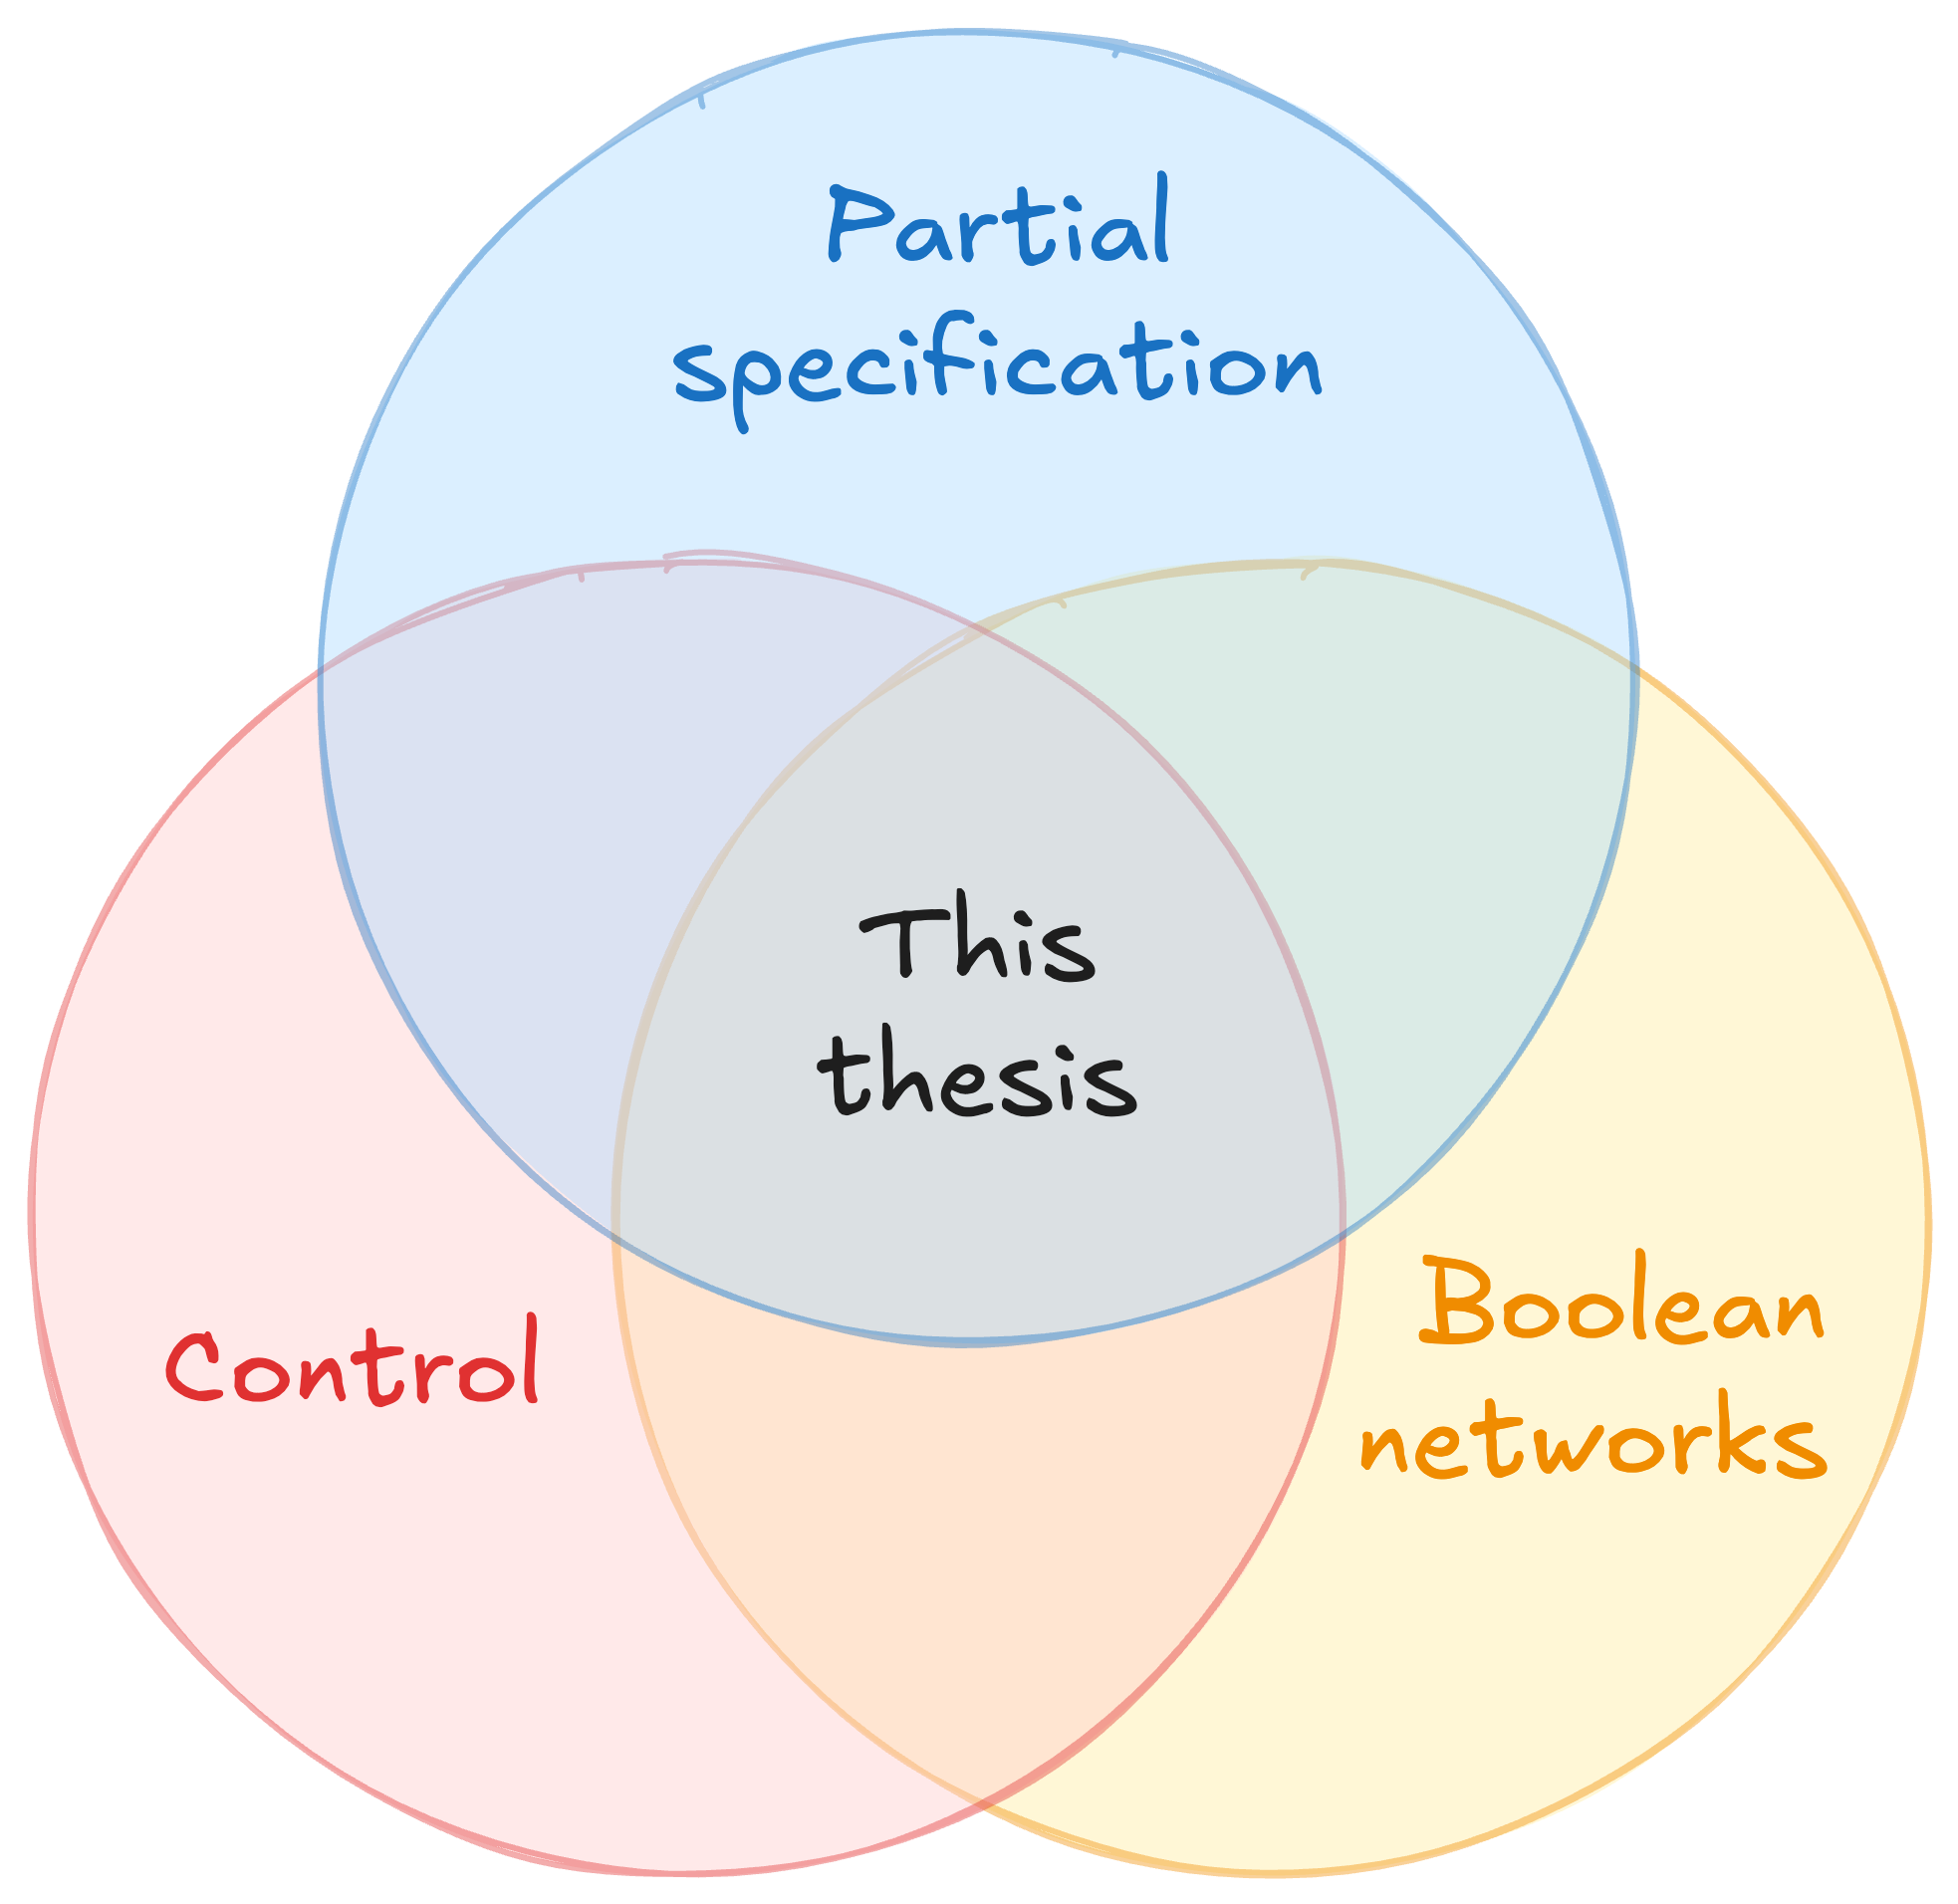
\includegraphics[width=0.5\textwidth]{Figures/topics.png}
    \caption{
        The confluence of concepts studied in this thesis. 
    }
    \label{fig:topics}
\end{figure}

The contribution of this thesis lies in its integration of three distinct concepts: control, asynchronous Boolean networks and systems with partial specification. Such a confluence has not yet been explored previously. The asynchronous Boolean networks are a well-studied model of system biology. Also, control is a commonly employed formal method in systems biology and the topic of controlling asynchronous BNs was already thoroughly studied as we describe in \autoref{s:control_of_bns}. On the contrary, the promising model of partially specified Boolean networks is just beginning its rise. Other formal methods such as attractor search~\cite{Benes2021, Roncalli2022}, bifurcation~\cite{Benes2022}, or parameter synthesis~\cite{Benes2023} are also being investigated only relatively recently.
 
The partial specification of BNs thus makes this work truly novel, although the specific approaches are often inspired by previously investigated intersections of the topics as we will see in the thesis. The objectives of this thesis are four-fold:

\begin{enumerate}
    \item Formally define control problem for partially specified Boolean networks
    \item Develop efficient methods that solve the control problem for partially specified Boolean networks 
    \item Bundle the developed methods to a software toolkit
    \item Demonstrate applicability for biological systems
\end{enumerate}

Now let us have a look at these goals in detail and describe in what parts of this thesis they are fulfilled.

\medskip

\noindent\PrimaryColor{\spacedlowsmallcaps{Goal 1 -- Problem definition.}}\hspace{3pt} Problem definition is an essential contribution of this work since the problem of \PBN{} control has not been formalized prior to my work. Several crucial aspects need to be considered for the problem definition. Firstly, attractors of the \PBN{} vary according to the interpretation. Therefore, searching for non-permanent perturbations that drive the network into a target attractor would be impossible for interpretations of unknown parts, where the given attractor is not present in the first place. Secondly, the practical realization of perturbations requires non-trivial effort; therefore, in a normal BN setting the number of perturbations is sought to be minimal. However, there is rarely a solution with a few perturbations in the partially specified setting, which would work for a big portion of interpretations. Thus, optimization criteria should be readjusted accordingly. 

The achievement of this goal is presented in \autoref{s:source_target_problem_definition} where we define \emph{source-target} control for \PBN{} which result is a relation of perturbations with interpretations for which they work as opposed to standard control goal where only minimal perturbation sets are returned. However, the landscape of attractors may change between interpretations~\cite{Benes2022}. That might cause a shift of target attractors that is not impeding from the cell reprogramming objective, but it is technically not allowed by a source-target control. This caveat is resolved by a more general notion of control -- \emph{phenotype} control which is defined in \autoref{s:phenotype_problem_definition} where only target traits are necessary to be known in advance.

\medskip


\noindent\PrimaryColor{\spacedlowsmallcaps{Goal 2 -- Efficient methods development.}}\hspace{3pt} As described before, the control problem for fully specified asynchronous BNs has been well-studied already. Therefore, after control for \PBN{} is formally defined, in theory, we could use the existing methods for asynchronous BN control to solve the problem for every interpretation distinctly. However, the number of these interpretations can be doubly exponential, meaning even a very efficient method for BN control would need to be run too many times to be handled in a realistic time. That is why seeking a novel, efficient approach for the partially specified setting is crucial.

Three methods were developed to solve the posed variants of the problem.

\begin{enumerate}
    \item Parallel one-step source-target control method for \PBN{} with semi-symbolic state space exploration and symbolic result which is described in \autoref{sec:target_semisymbolic}~\cite{Brim2021}
    \item One-step, temporary, and permanent source-target control for \PBN{} with symbolic state space exploration and symbolic result which are described in \autoref{sec:ostp_symbolic}~\cite{brim2022}
    \item Permanent phenotype control method with symbolic state space exploration for \PBN{} and result requiring explicit enumeration which is described in \autoref{chapter:phenotype_control_psbn}~\cite{Benes2023b}
\end{enumerate}

The aforementioned sections present algorithms, and simple (i.e., quantitative) demonstrations of them.

\medskip

\noindent\PrimaryColor{\spacedlowsmallcaps{Goal 3 -- Software toolkit for methods.}} \hspace{3pt} In order to make the developed methods publicly available, they were incorporated to the BioDivine toolkit~\cite{Barnat2009}. A library in Rust based on AEON tool~\cite{aeon} was developed to make methods fast and performant. Later, the library was wrapped into Python language as part of AEON.py tool~\cite{aeonpy}. This helps to make the methods more convenient to work with for the wider scientific audience because the language is easier to learn and offers popular notebook environments such as JuPyter~\cite{Barba2021}. The Python version also has become part of the CoLoMoTo Interactive Notebook tools~\cite{Naldi2015,Levy2018}. Finally, the control functionality was also embedded into AEON web application~\cite{Vesely2025}. The software technical specification and solved challenges are in detail described in \autoref{chapter:software}.

\medskip

\noindent\PrimaryColor{\spacedlowsmallcaps{Goal 4 -- Applications to biological systems.}}\hspace{3pt}
Finally, since Boolean network control is closely connected to cell reprogramming, we demonstrate that the developed methods address the original biological motivation of this thesis. In addition, we show that control can also serve as a tool for model refinement. Both applications, together with case studies illustrating their utility, are presented in \autoref{chapter:applications}.

\section{Thesis structure}

As mentioned before, this thesis covers multiple interlaced themes. Thus, it is important for the reader to recognize what aspects are considered while reading this thesis, especially distinguishing where only fully specified Boolean networks are discussed and where their partial specification is assumed. To help with that, a switch from the context be indicated by accompanying figure in the margin of the text, similar to one in \autoref{fig:topics}. Also, in the following text we provide a brief guidance on the structure of the thesis and what is covered in each chapter.

\autoref{chap:prelim} describes all necessary preliminaries to understand the basic problematic of the fully specified Boolean networks. Regulatory networks, which are an essential basis for BNs and also \PBN{s} are described at first (\autoref{s:reg_net}). Then, all motivation and formal definitions related to fully specified BNs are introduced (\autoref{section:boolean-networks}). After that, the control problem for BNs, is described, including technical differences between all variants of the problem (\autoref{s:control_of_bns}). Finally, the notion of partially specified Boolean networks is introduced (\autoref{s:psbn}), including the motivation for this model and the technical details of it.

\autoref{chap:sota} is about the state of the art in the field of control of Boolean networks. It covers the methods for control from the most general classes of the systems to the systems most similar to the \PBN{}s. First, it describes roots of the control theory in terms of discrete systems (\autoref{sec:controlDiscrete}) and incompletely specified systems (\autoref{sec:controlPartiallySpecified}). Then, it describes the methods for control of fully specified BNs from the simplest synchronous BNs (\autoref{sec:controlSynchronous}) to the more complex asynchronous (\autoref{sec:controlAsynchronous}) and most-permissive BNs (\autoref{sec:controlMostPermissive}). Finally, it describes how the control problem for BNs can aid the problem of model refinement (\autoref{sec:controlInference}) and a comparison of the software tools for control of BNs is given (\autoref{sec:relatedTools}).

\autoref{chapter:source_target_control} provides the problem definition of source-target control problem for \PBN{} (\autoref{s:source_target_problem_definition}) and then it also shows two methods that solve this problem. The first one, semi-symbolic and parallel uses only the most trivial one-step perturbation (\autoref{sec:target_semisymbolic}). The later developed fully symbolic method is capable of one-step, temporary and permanent perturbations (\autoref{sec:ostp_symbolic}). Finally, these two methods are discussed and compared (\autoref{sec:control_evaluation}).

\autoref{chapter:phenotype_control_psbn} describes the problem of phenotype control for \PBN{} (\autoref{s:phenotype_problem_definition}) and a method to solve it (\autoref{sec:phen_control_method}). The method is based on the same symbolic state space exploration as the one for source-target control. Finally, the method is evaluated on several middle-sized \PBN{}s (\autoref{sec:phen_control_evaluation}) in terms of performance and the quality of the results. 

\autoref{chapter:software} describes the software implementation of the presented methods. First, the software architecture is described (\autoref{sec:software_architecture}), including the main libraries and their functionalities (\autoref{sec:core_packages}). Then, the web application for control of \PBN{} is presented (\autoref{sec:aeon_web_app}), followed by the description of the Python package (\autoref{sec:python_package}).

\autoref{chapter:applications} is about the applications of the developed methods for control of \PBN{}. Firstly, it described the primary motivation for this work -- the problem of cell reprogramming in regenerative medicine (\autoref{sec:cell_reprogramming}). Then, it shows an example of \PBN{} control application for cell reprogramming on a specific example of a myeloid cell (\autoref{sec:myeloid_case_study}). After that, a more general workflow of how the control of \PBN{} can be used to design a therapy or to refine the model is described (\autoref{sec:control_workflow}). Finally, this workflow is shown on the second case study that is focused on the MAPK signalling pathway and demonstrates the control-guided model refinement (\autoref{sec:mapk_case_study}).

Finally, \autoref{chapter:conclusion} summarizes the main contributions of this thesis and discusses possible future directions for research in this area.